%!TEX root = memoria_duocode_interfaz.tex

Todos nos hemos ayudado y colaborado durante este proyecto pero en esta sección explicaré las tareas que yo, Johana Gabriela Ferreira Yagua, específicamente he realizado.

\begin{itemize}
\item
Al empezar el proyecto, una de las principales cosas que teníamos que decidir era qué tipo de servicio web utilizar. Yo me encargué de buscar información sobre RCP y sus ventajas y desventajas para compararlas con SOAP y REST.

\item
Intenté hacer dos ejemplos de servicio web REST, uno utilizando Spring con eclipse y otro con Jersey para comparar cuál era más sencillo de utilizar. En ambos casos el ejemplo utilizado fue el algoritmo de factorial.

\item
Hicimos una reunión, presidida por mí, para crear un diseño inicial del modelo entidad-relación de la base de datos.

\item
Me encargué de pasar el diseño del modelo entidad-relación a ordenador y de hacer los cambios necesarios.

\item
Después de tener el modelo entidad-relación, creé la base de datos, las tablas con sus correspondientes atributos y las relaciones con \texttt{phpMyAdmin}.

\item
Hice la población de la base de datos con información válida para realizar las pruebas.

\item
Creé varias clases que representan el modelo de la aplicación, sus correspondientes \texttt{`mappers'} para acceder a la base de datos~\ref{sec:accesoBD} y las funciones para los distintos verbos de los recursos REST (GET, POST, PUT y DELETE):

\begin{itemize}
\item
Todo lo relacionado con los usuarios, incluyendo el GET de un usuario específico, que aporta toda la información registrada del usuario en la aplicación (historial de ejercicios, candidatos propuestos, ejercicios favoritos, lecciones completadas y votos a otros candidatos). Aparte del \texttt{`mapper'} de usuario, existen otros dos \texttt{`mappers'}, uno para las lecciones que ha completado el usuario y otro para los votos que ha realizado a distintos candidatos.

\item
Todo lo relacionado con los candidatos, incluyendo en el PUT la diferenciación si se trata de un usuario común o de un administrador: en el primer caso el usuario sólo puede modificar el voto a positivo o negativo; en el segundo, además de tener esa capacidad, puede gestionar el ejercicio dándolo por válido o por rechazado.

\item
Todo lo relacionado con los lenguajes.

\end{itemize}
    
\item
Realicé los prototipos en papel para tener una idea de cómo queríamos que fuese el aspecto visual de la aplicación y su estructura interna.

\item
Realicé los primeros ejemplos con HTML y CSS con la estructura anteriormente definida e hice que la sección de información del usuario fuese fija para que estuviese presente en todo momento.

\item
Hice pruebas con distintas combinaciones de colores y fondos, por ejemplo:

\begin{figure}[H]
\begin{center}
\makebox[\textwidth]{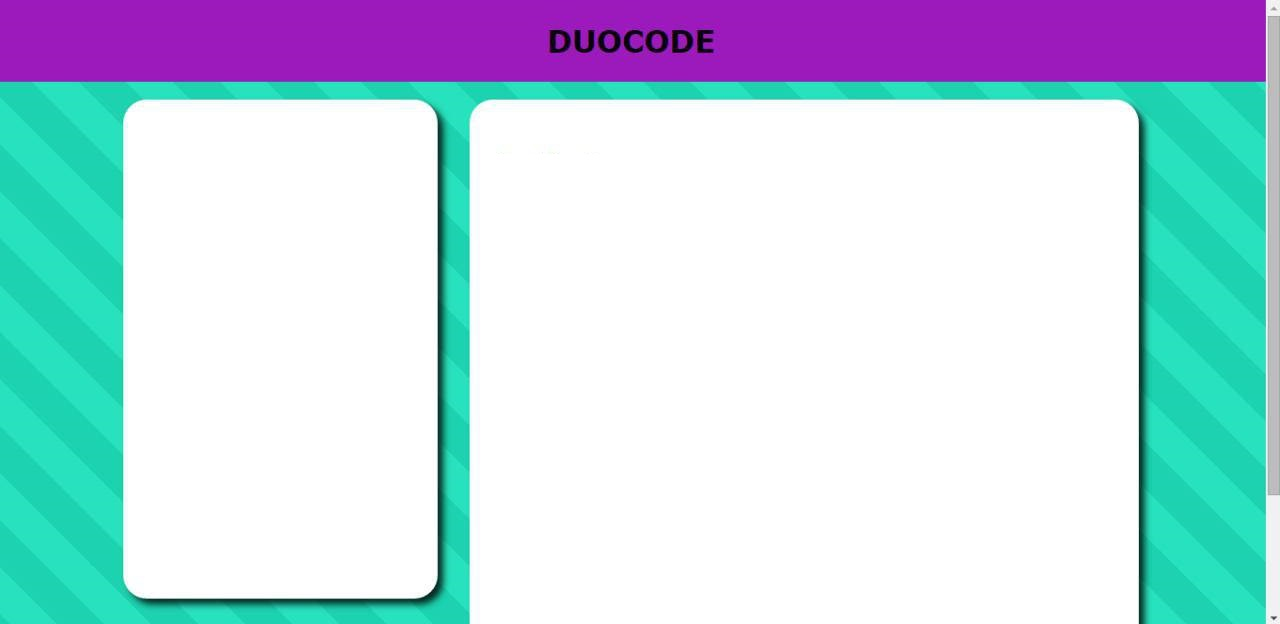
\includegraphics[scale=0.4]{images/color1}}
\end{center}
\end{figure}

\begin{figure}[H]
\begin{center}
\makebox[\textwidth]{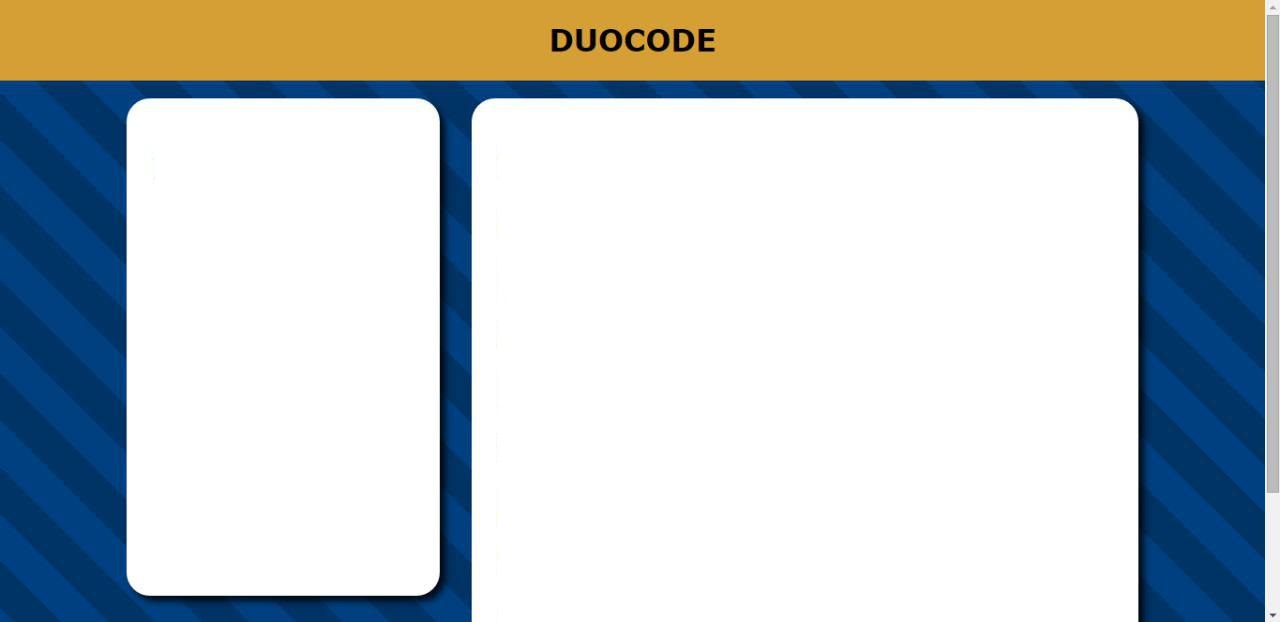
\includegraphics[scale=0.4]{images/color2}}
\end{center}
\end{figure}

Finalmente, pensé en probar con la paleta de colores \texttt{Monokai} ya que es muy utilizada en programación; esta fue la definitiva.

\item
Incorporé con Bootstrap un pop-up explicativo al iniciar cada lección, el cual está accesible una vez iniciada la sesión por si el usuario quiere volver a verlo. También hice un pop-up explicando qué significa enviar un ejercicio como candidato cuando se da esta opción.

\item
Hice la vista de favoritos del usuario. Para que no saliese demasiada información en esta vista, al principio sólo se muestra el título de los ejercicios marcados como favoritos y sus correspondientes lenguajes de programación en los que fueron marcados. Usé la opción \texttt{Collapse} de Bootstrap para mostrar y ocultar el código de los ejercicios cuando el usuario seleccione uno de ellos.

\item
Hice la vista de candidatos de un usuario basándome en la de favoritos para buscar consistencia visual en la web.

\item
Hice la vista de lenguajes que se muestra al entrar en la web. Para que un usuario no pueda elegir el mismo lenguaje de programación en las listas ``Lenguaje que sé'' y ``Lenguaje que quiero aprender'' utilicé AngularJS.

\item
Me encargué de realizar las peticiones al servicio web para saber las lecciones que corresponden a un tema.

\item
Me encargué de realizar las peticiones al servicio web para obtener la información del usuario:

\begin{itemize}
\item
Nombre y foto.
\item
Número de candidatos enviados.
\item
Número de ejercicios marcados como favorito.
\end{itemize}

\item
Me encargué de realizar las peticiones al servicio web para obtener los candidatos de un usuario.

\item
Me encargué de realizar las peticiones al servicio web para obtener los favoritos de un usuario.

\item
Hice que en el pop-up explicativo de las lecciones saliera la información correspondiente.

\item
Añadí la función de iniciar sesión con Google+ y con Facebook mediante la estructura creada por Julián.

\item
Añadí la función de compartir con Facebook el éxito tras superar una lección.

\item
En la memoria me encargué de hacer la sección Resumen~\ref{sec:res} y su traducción al inglés~\ref{sec:abs}.

\item
En la memoria me encargué de hacer la lista de palabras clave y su análogo en inglés, keywords.

\item
En la memoria me encargué de hacer la sección Requisitos y base de datos~\ref{sec:req}.

\item
En la memoria me encargué de hacer la sección Manual de usuario~\ref{sec:manual}.

\item
En la memoria me encargué de hacer el apéndice Especificacion de requisitos~\ref{app:req}.

\end{itemize}